\section{Method} \label{sec:method}

%Currently, the IEC Wave Resource Assessment technical specification (TS) focuses on quantifying resource parameters that are important to characterizing the resource across different spatial scales (i.e., three "classes" of resource assessment), but it provides little guidance on how to sum the theoretical resource for a region or site of interest. This is because this technical specification is focused primarily on characterizing the resource for feasibility studies (class 1 and 2) and quantifying the resource for designing projects where technologies are known (class 3). At the feasibility level, omni-directional wave power serves as a useful metric for quantifying the opportunity for wave energy development. When conducting array design, the TS states that ``the effects of the WEC array on wave propagation should be included in the numerical model. Any modifications made to the numerical model to account for the effects of a WEC array shall be documented and justified.'' This is important guidance that effectively accounts for wave directionality, but it is not practical or feasible when performing large-scale theoretical resource assessments for arbitrary devices. Instead, the approach used here skips the complexity of simulating many (thousands to millions or more?) of individual WECs extracting energy, and instead treats the line as a `perfect' array that extracts all of the incoming energy. By using a line-integral (dot-product), we are accounting for the directionality of waves (i.e., the `shadowing effect' of arrays) that is called for in the standards. Thus, the line-integral approach effectively accounting for the `shadowing effect' that is required by the IEC TS, and therefore this approach is consistent with it.


\begin{figure}[ht]
\centering
%\includegraphics[width=0.9\linewidth]{../diagram/EEZ_contour03_edit01.png}
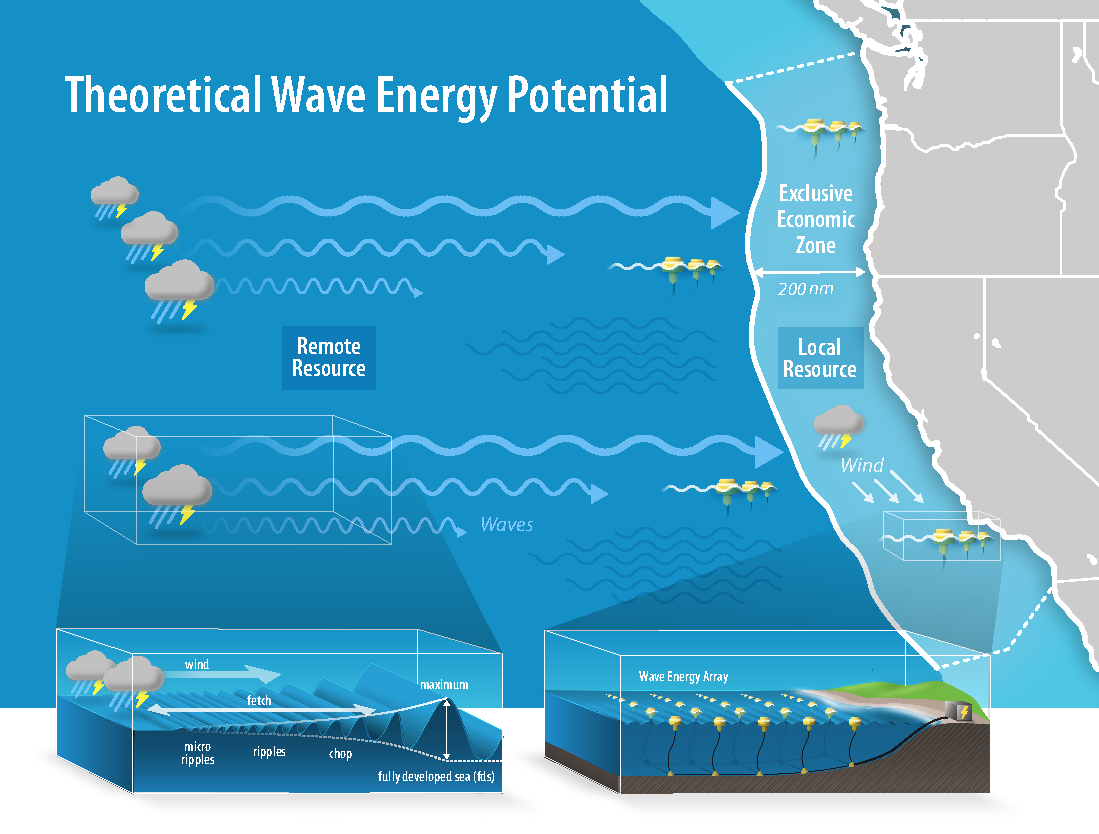
\includegraphics[width=\linewidth]{../fig/NREL-water-NatureEnergyGraphic-Levi-FY21-jfrenzl-v5.png}
%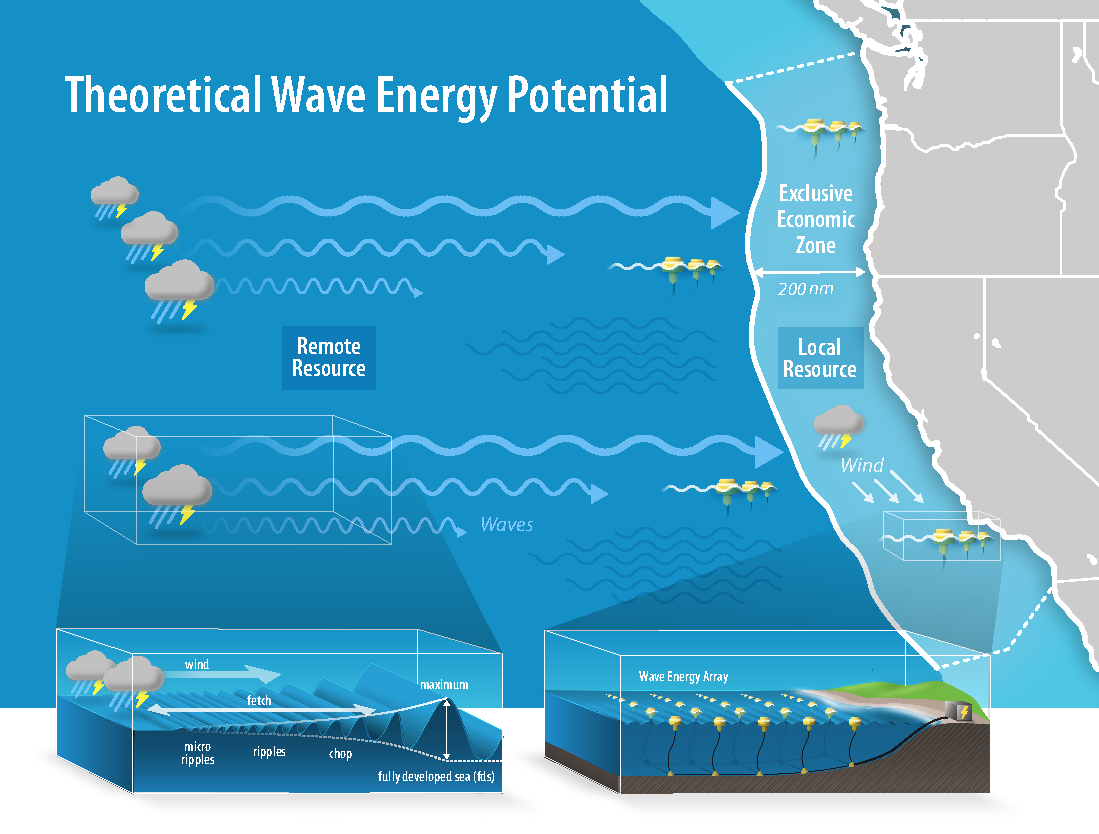
\includegraphics[width=\linewidth]{../fig/NREL-water-NatureEnergyGraphic-Levi-FY21-jfrenzl-v5.pdf}
\caption{A diagram depicting the U.S. West Coast's wave energy resource. Insets show the generation of waves by storms (left), and a schematic of a hypothetical wave array (right).}
\label{fig:diagram:west-eez}
\end{figure}

The proposed methodology eliminates ``double counting'‘ and includes all sources of wave energy that are legitimately a portion of the region's resource. Specifically,

\begin{enumerate}
    \item This methodology follows IEC TS-101 standards for numerical model setup, configuration, and validation. The IEC standards provide internationally accepted guidelines for model setup and procedures for validation. In addition to the IEC requirements, the model must also be configured to output the source terms, so that the `local resource' (defined below) can be computed.
    
    \item The total wave resource is defined as the sum of the remote and local resource (Figure \ref{fig:diagram:west-eez}). The majority of existing wave resource assessments have considered the remote resource only. To our knowledge, this is the first work to define and propose including the local resource in the total resource estimate. The inclusion of the local resource is a means for accounting for the 'recovery' of the wave-field downstream of where energy is extracted.
    
    The remote resource is defined as the wave energy propagates into the domain. The remote resource can be calculated utilizing a one-way dot-product at the boundary of the domain. This approach has been used in several previous wave resource assessments \citep{gunnQuantifyingGlobalWave2012, hemerRevisedAssessmentAustralia2017, regueroGlobalWavePower2015}. This is a fundamental component of wave resource assessment because it avoids double counting.
    
    The local resource is the wave energy that is generated by winds within the boundary of the domain. Adding this local energy resource directly accounts for wave energy created by winds inshore of the chosen boundary. To the authors' knowledge this has not been considered in previous resource assessments.

    \item Extend the assessment to the edge of the region's legal boundaries. Based on Article 56 of the U.N. Law of the Sea — which states that ``in the exclusive economic zone, the coastal State has sovereign rights [to] the production of energy from the water, currents and winds'' — we propose that national resource assessments should utilize the exclusive economic zone (EEZ) as the domain over which wave energy resource totals are calculated (United Nations General Assembly 1982). We also note that the method should not count wave energy fluxing across the boundary between the two regions, because doing so would amount to double counting that portion of resource for both regions.
\end{enumerate}


\note{We need to introduce the 'inner-shelf' resource somewhere here...}

\subsection{Numerical Model} \label{sec:method:model}


Wave resource assessments typically rely on the use of wave model `hindcasts' to estimate the history of the wave field over the region(s) of interest, and then to compute estimates of the theoretical resource from the model output. Wave hindcasts provide long term time series at high spatial and temporal resolution. In this work all wave climate hindcasts are simulated using WAVEWATCH III\textregistered v5.16 \citep{tolmanDistributedmemoryConceptsWave2002,tolmanwavewatch}.

WAVEWATCH III\textregistered (hereafter WW3) is a  well established numerical model that has been implemented successfully in many previous wave resource assessments \citep[e.g.,][]{garcia-medinaWaveResourceAssessment2014,hemerRevisedAssessmentAustralia2017,yangWaveModelTest2017}.
WW3 solves the five-dimensional action balance equation:

\begin{align}
  \frac{d N}{d t} = \frac{\Src{tot}}{\sigma} = \frac{1}{\sigma}\left ( \Src{in} + \Src{ds} + \Src{brk} + \Src{nl} + \Src{bot} \right )
  \label{eqn:actionbalance}
\end{align}
where $N(t,x,y,\sigma,\theta) \equiv D/\sigma$ is the wave action, $D$ is the variance spectrum, $t$ is time, $x$ and $y$ are the spatial coordinates, $\sigma$ is the radian frequency, and $\theta$ is the direction of wave propagation.
The wave action is conserved in the absence of sinks and sources of energy, their combined effect is represented as $\Src{tot}$.

In this study we implement the ``ST4'' physics package option in WW3 to simulate wind energy input ($\Src{in}$) and dissipation due to whitecapping ($\Src{ds}$) \citep{ardhuinObservationSwellDissipation2009}.
The wind forcing is taken from NOAA's Climate Forecast System Reanalysis (CFSR) \citep{sahaNCEPClimateForecast2010}. The non-linear quadruplet interactions ($\Src{nl}$) are modeled with the Hasselmann and Hasselmann (\citeyear{hasselmannComputationsParameterizationsNonlinear1985}) formulation. Bottom friction ($\Src{bot}$) and depth induced wave breaking ($\Src{brk}$) are modeled with the JONSWAP Hasselmann etal. \citeyear{hasselmannMeasurementsWindwaveGrowth1973} and Battjes and Janssen \citeyear{battjesEnergyLossSetup1978} models, respectively. Finally, the effect of sea ice is considered by using a time varying mask based on the ice coverage fields from CFSR. Default parameters are used for all formulations. The wave spectrum is discretized with 24 equally spaced bins in $\theta$ space and 29 logarithmically spaced frequency bins from 0.035Hz to 0.5Hz with an increment factor of 1.1. The WW3 simulations span a 31-year period from 1 January 1980 to 31 December 2010.

Model grids and bathymetry come from the NOAA NCEP hindcast Phase 1 mosaic-model \citep{chawla2011wavewatch,chawla201230}. In this system a global model (0.5$^{\circ}$ resolution) drives regional models (10" - 4" resolution) providing complete coverage over the U.S. EEZ with higher resolution focused on shallower waters. This model was reimplemented to store wave spectra and source terms at a high resolution. This model configuration is mostly aligned with the IEC TS 62600-101 requirements for a reconnaissance class resource assessment.

Model output is collected at the U.S. EEZ around Alaska (excluding the Arctic Coast), Atlantic Coast, Caribbean Coast (Puerto Rico and U.S. Virgin Islands), Gulf Coast, Hawaii (excluding the Papah$\bar{\text{a}}$naumoku$\bar{\text{a}}$kea Marine National Monument), and the West Coast. Full variance spectra are stored at the U.S. EEZ boundary (at 200 nmi from shore, and along EEZ `borders' with other nation's). Inside the EEZ, directionally integrated source term output is collected at lines of equal distance from shore from 18.5 km (10 nmi) to 351.9 km (190 nmi) every 18.5 kms. Both output types are collected at hourly intervals every 1/6$^{\circ}$ along the defined lines.

In WW3, as it is customary in third-generation spectral wave models, the waves are computed over a specified spectral width after which a spectral tail is appended to represent the energy in the high frequencies \citep[e.g.][]{ardhuinObservationSwellDissipation2009}. The source terms are integrated over the range where the wave spectrum is actively simulated when estimating the local resource as discussed in Section \ref{sec:method:calc:local}.

\subsection{Calculate Resource Totals} \label{sec:method:calc}

In this work we propose that the total theoretical wave resource, $R_T$, be defined as a sum of `remote' and `local' components:
\begin{align}
  R_T = R_R + R_L
\end{align}
The remote resource, $R_R$, is the piece of the wave energy resource that has previously been defined as the total wave resource \citep{gunnQuantifyingGlobalWave2012,EPRIwaveresource2011}.%, while the local resource, $R_L$, has not previously been included in wave resource assessments.

\subsubsection{Remote Resource} \label{sec:method:calc:remote}

The remote resource is computed as a line-integral of the wave energy that fluxes toward the coastline across the EEZ boundary when it is bordered by international waters. 

\begin{align}
  R_R = \rho g \int_{\ell}\iint \delta \, c_g(f) \, \bar{D}(f,\theta) \d f \d \theta \d l
\label{eqn:RR}
\end{align}
Where $c_g(f)$ is the wave group velocity, $\ell$ is the integration contour, and $\delta$ is the directionality coefficient which we take to be $\delta = \cos(\theta_n - \theta)$ for waves propagating toward the coastline, and $\delta = 0$ otherwise. 
$\theta_n$ is the direction normal to the contour pointing toward the shoreline. 
This `one-way' condition ensures that waves propagating offshore are not {\em subtracted} from the total \citep[]{gunnQuantifyingGlobalWave2012}.
%A detailed rationale for the one-way approach is included in appendix \ref{appendix:one-way-method}.
The over-bar denotes a time-average of the wave-variance spectrum over the 31-year period from Jan. 1 1980, through Dec 31, 2010.

In this work, the integration contour $\ell$ is the segments of the U.S. EEZ that separate U.S. EEZ waters from the open-ocean (hereafter the `EEZ boundary'; thick black line in Figure \ref{fig:diagram:west-eez}), and does not include the EEZ segments that separate one nation's EEZ from that of a neighbor (hereafter the `EEZ borders'; thin dashed lines) \citep[]{flandersmarineinstituteMaritimeBoundariesGeodatabase2018}. This is because wave-energy that fluxes across EEZ borders will be counted by the nation from which that resource originated, and should not be counted a second time where it fluxes across the border into a neigboring nation's EEZ.


\subsubsection{Local Resource} \label{sec:method:calc:local}

%While neglecting the local resource may be reasonable for small projects, the fact that it typically has been implicitly ignored has raised legitimate questions about the validity of earlier theoretical resource assessment methodologies, which has led to skepticism and confusion. 
The local resource is computed as an area-integral of all wave source- and sink-terms, except for bottom friction:

\begin{align}
  R_L &= \rho g \int_{EEZ}\iint \left ( \bar{S}_{in} + \bar{S}_{ds} + \bar{S}_{nl} \right ) \d f \d \theta \d A
\label{eqn:RL}
\end{align}
where $dA$ is differential-area integral of the source terms.
%Since the model results are output in spherical coordinate system, the coordinates were transformed using an Albers equal area projection before performing the area integral. 
%By performing these projections on a region-by-region basis with carefully chosen projection parameters, this approach introduces $<1\% $ local distortion at the edges of the largest regions (Alaska), and therefore introduces a $\ll 1\%$ error in the total estimate of $R_L$.

Note that the depth-induced wave breaking ($S_{brk}$) and bottom friction ($S_{bot}$) terms from \eqref{eqn:actionbalance} are neglected in \eqref{eqn:RL}.
These terms are neglected because they close \eqref{eqn:actionbalance} by dissipating all of the energy that arrives at the shoreline (the model does not include wave reflection). Including these terms, therefore, would be contrary to the purposes of resource assessment, becase the goal is to calculate how much of that energy exists \textit{before} it dissipates at the shoreline.

It should be noted that the white-capping term ($\bar{S}_{ds}$) is negative, and the non-linear term ($\bar{S}_{nl}$) -- which transfers energy from high- to low-frequency -- is also negative because the model does not solve the highest frequencies.
Based on these facts, it is tempting to assume that wave energy originating from the large positive term $S_{in}$ could be absorbed prior to these other terms dissipating it because this approach would yield a significantly larger local resource. Doing so, however, is scientifically questionable for three reasons. First, the spatial and temporal scales at which $S_{in}$ delivers energy to the wave field is similar to the scales at which $S_{ds}$ removes it. In other words, significant white-capping and dissipation occurs when winds generate waves. Second, the details of wave-generation is an active area of research, with large uncertainty associated with each term's magnitude. The sum of the terms, on the other hand, is relatively well constrained as demonstrated by the performance of wave models in general (i.e., via wave-model validation studies \citep[e.g.][]{ardhuin_semiempirical_2010,van_vledder_source_2016}). Third, there are significant practical questions about extracting small-wave energy (i.e., at the scales that the majority of $S_{in}$ energy exists) across sufficiently large spatial-area for the energy to be sizable. Therefore, it makes sense to include the $S_{nl}$ term in order to properly quantify the degree to which low-frequency waves are generated by winds.

There is certainly an inherent tension here between, ``including the local resource in order to provide a complete assessment of the {\em theoretical} wave resource'', and assuming that some pieces of the wave source terms (wind input) are inaccessible on {\em practical} and {\em technical} feasibility grounds. In other words, some might argue that including the negative source terms belongs in a technical or practical resource assessment. However, we argue that including $R_L$ as defined here is already a relatively optimistic proposal. 
The task of quantifying any resource, including the theoretical resource, involves making some assumptions about what is realistic and what is not. 
Perhaps more importantly, until we have a better understanding of the magnitude (i.e., uncertainty) of the individual terms, and we have technologies that show promise for extracting high-frequency energy at spatial and temporal scales between wind-input and non-linear transformation to lower frequency, neglecting these negative terms seems scientifically dubious.

\paragraph{Discussion on methodological changes related to $R_L$}

This piece has not typically been considered in wave resource assessments. This is most likely because it is obvious that for projects within 10 to 20 miles of shore - where it seems reasonable to assume the majority of projects will be for the next several decades - $R_L \ll R_R$. However, when we are taking the perspective of an assessment of the nation's resource - which according to the U.N. law of the sea legally extends to the edge of the U.S. EEZ - $R_L$ is an important piece of the total energy available. By accounting for this term, this methodology directly incorporates the energy added to the wave field over that area. While it does not directly address the question ``how quickly will the wave-field re-energize down-wave from a wave farm?'' It does explicitly include this energy.

However, because the source terms in \eqref{eqn:RL} depend on the sea-state and the sea-state depends on energy extracted ``up-wave'', there is ambiguity in estimating $R_L$ related to where and when wave energy is extracted by WECs. To address this, we calculate two estimates of $R_L$. The first, `natural local resource' ($R_{L_\circ}$) is calculated from the source-terms where waves from the global domain propagate freely throughout the regional domain (the EEZ). The second, `potential local resource' ($R_{L_*}$) is calculated from the source-terms when no wave energy propagates across the EEZ boundary. In other words, this is a `lake case' that only contains waves generated by winds within the regional domain.

In all cases we examined, $R_{L_*}$ was found to be greater than $R_{L_\circ}$.
%(see Appendix \ref{appendix:flux-vs-area} for details)
In the sense that $R_L$ is meant to be an estimate of the maximum energy available, this suggests that $R_L$ could be defined as being equal to $R_{L_*}$. However, the scenario of removing all wave energy from the wave field at the edge of the EEZ is so hypothetical that it seems unrealistic to use this value to define $R_L$. Therefore, we choose to treat these two estimates of $R_L$ as an uncertainty range for the value.

It is worth noting that -- though a line-integral that accounts for directionality of the wave flux (a vector quantity) is applicable for estimating $R_R$ \eqref{eqn:RR} -- directionality is not important to estimating $R_L$ correctly in \eqref{eqn:RL} (i.e., all directions are weighted equally). This is because the source terms are scalar quantities that are functions of direction per unit-area, and therefore an area-integral applies.
%This can be understood by considering the hypothetical case of an array of WECs that covers the entire EEZ. The wave energy that is added locally within the EEZ will be absorbed -- regardless of it's direction -- by the array before it reaches the edge of the EEZ where a line-integral would be appropriate (i.e., when directionality is important).


%%% Local Variables:
%%% TeX-master: "wave_res"
%%% End:
